
The kinematical cuts such as $\pt$, $\eta$ of lepton and jets, missing transverse energy (\MET),
transverse mass of leptonically decaying W Boson (MT) etc are used to enhance the signal contribution thus 
affect the exclusion limit on the ${\cal{BR}}(t \rightarrow b H^+)$.
Different combinations of these cuts affect the final event yields as well as the shape of the
\mjj distribution. For \mujets channel, some of the combinations of cuts are 
explored as discussed in the next section. Similar results are expected for \ejets channel.

\subsection{Di-jet Mass Resolution for Different MET and MT}
The combination of \MET and MT cuts are expected to reduce those background where there is 
no neutrino at the parton level such as QCD, VV, $Z/\gamma+ jets$. The \mjj distribution for different combination of \MET and MT are shown in Figure~\ref{fig:mjj_met_mt_mu} with corresponding statistical parameters in 
Table~\ref{tab:mjj_met_mt_mu}. From Table~\ref{tab:mjj_met_mt_mu}, it can be seen that the additional MT cut 
is not improving \mjj resolution. Also, it can be seen from Fig~\ref{fig:limit_cutset} 
that the exclusion limit without any MT cut is better. In view of this, no MT cut is applied in this analysis.

\begin{figure}
\begin{center}
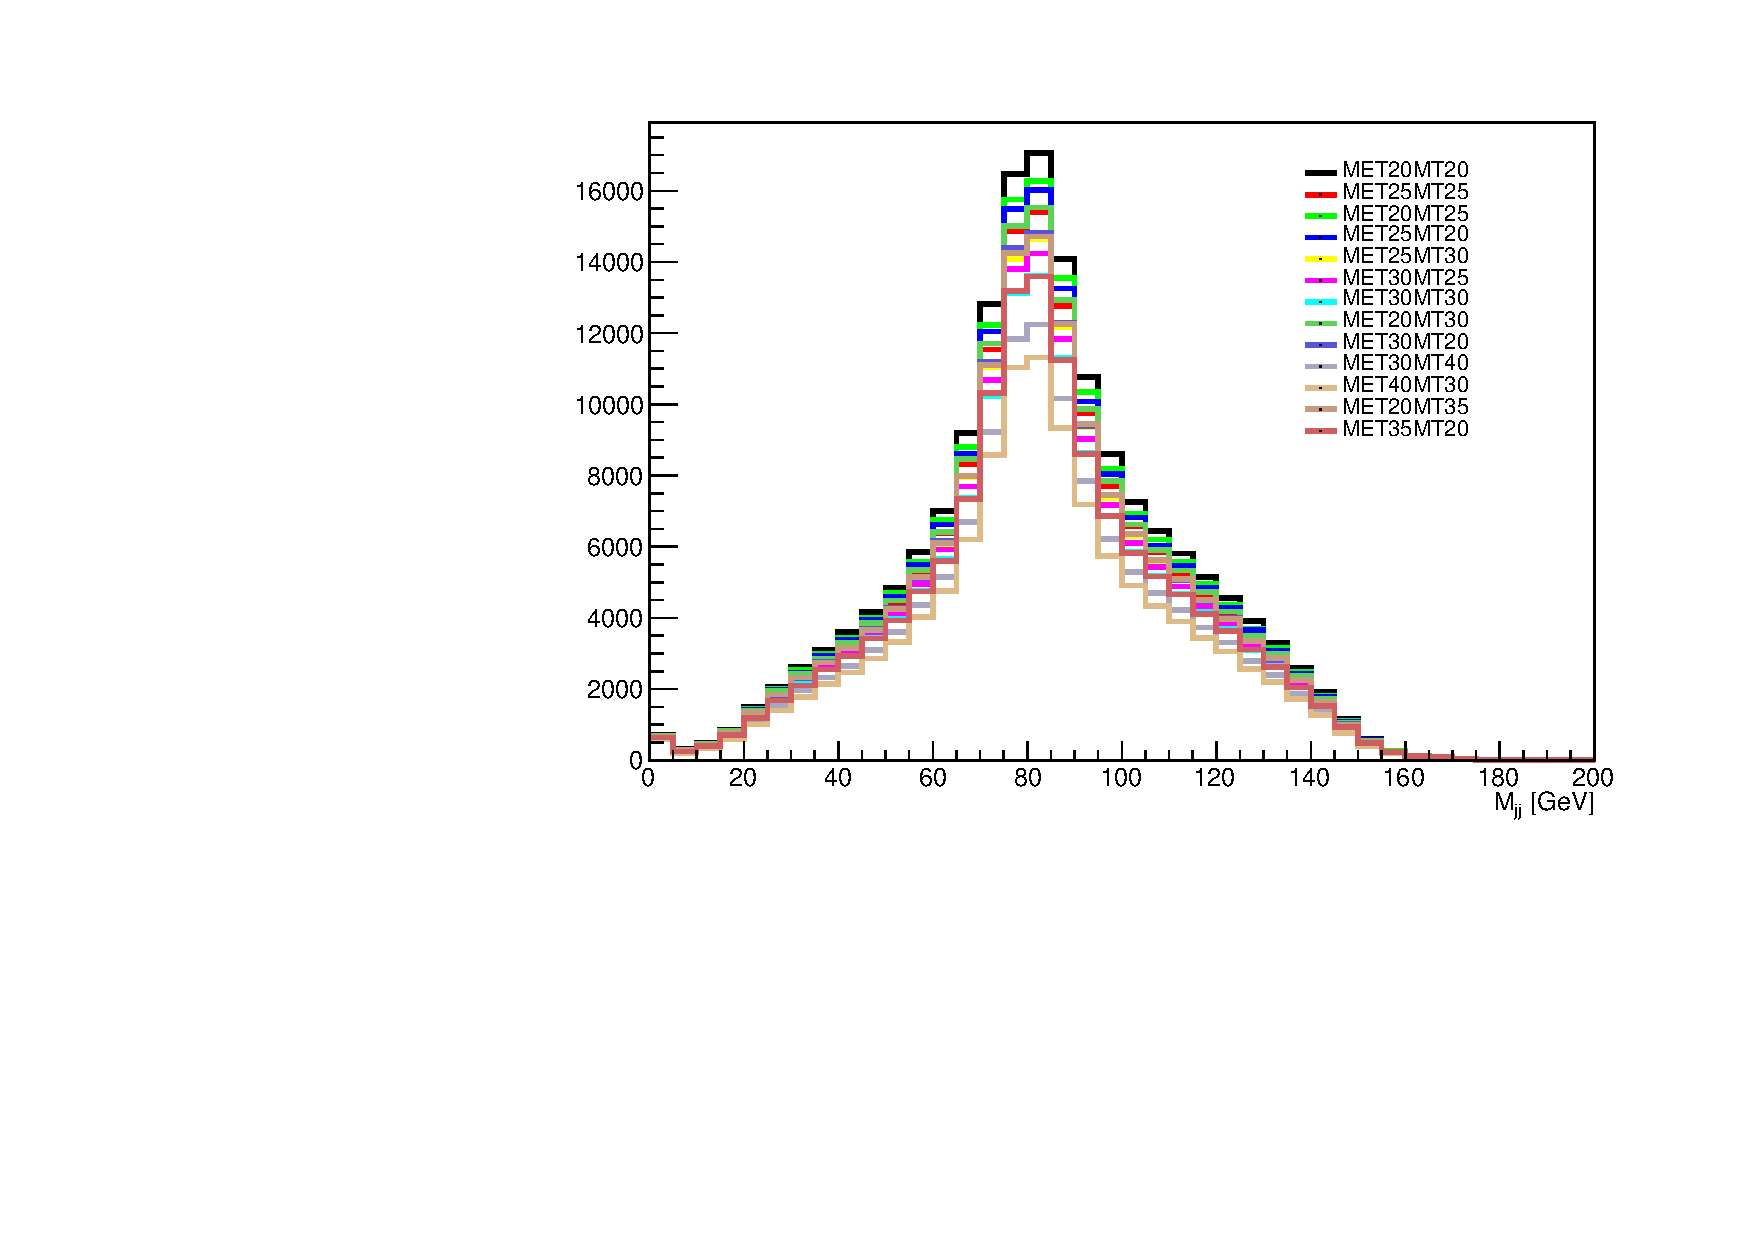
\includegraphics[width=0.70\textwidth]{Image/Limit/mjj_met_mt_mu.pdf}
\caption{The \mjj distribution for the different combinations of \MET and MT from \ttjets process
    in \mujets channel. The mean, RMS and resolution of these distributions are shown in 
    Table~\ref{tab:mjj_met_mt_mu}. On one hand the MT cut is not improving the resolution of \mjj and on 
    the other hand, it is reducing the number of events.}
\label{fig:mjj_met_mt_mu}
\end{center}
\end{figure}

\begin{table}[tbp]
    \caption{For  \ttjets process, statistical parameters from \mjj 
        distributions for various combinations of \MET and MT cuts, keeping all other 
        selection cuts on various objects same, in \mujets channel. For all the
        combinations the mean and sigma are almost same. The \mjj distribution has
        highest number of events for the lowest values of \MET = 20 GeV and MT = 20 GeV.}
\begin{center}
\begin{tabular}{|c|c|c|c|c|c|}\hline
\MET(GeV)& MT (GeV) & Events & Mean (GeV) & RMS (GeV) & Resolution($\sigma$) (GeV)\\ \hline
    20 &  20 & 180851 & 83.64 & 28.06 & 12.02\\
25 &  25 & 163776 & 83.53 & 28.11 & 12.05\\
20 &  25 & 136720 & 83.59 & 28.08 & 12.06\\
25 &  20 & 134359 & 83.57 & 28.07 & 11.97\\
25 &  30 & 156301 & 83.51 & 28.15 & 12.15\\
30 &  25 & 152340 & 83.49 & 28.16 & 12.03\\
30 &  30 & 145717 & 83.44 & 28.19 & 12.07\\
20 &  30 & 165511 & 83.51 & 28.12 & 12.13\\
30 &  20 & 158429 & 83.52 & 28.10 & 11.99\\
30 &  40 & 131690 & 83.29 & 28.27 & 12.18\\
40 &  30 & 122343 & 83.36 & 28.25 & 12.10\\
20 &  35 & 157343 & 83.48 & 28.15 & 12.14\\
35 &  20 & 145775 & 83.48 & 28.15 & 12.01\\\hline
\end{tabular}
\end{center}
\label{tab:mjj_met_mt_mu}
\end{table}

\subsection{Exclusion Limit for Different Set of Cuts}
The cut optimization is performed on the various sets of kinematical cuts as shown in Table~\ref{tab:limit_cutset}. The 
exclusion limit on the ${\cal{BR}}(t \rightarrow b H^+)$ for these set of cuts is calculated for different mass of the 
charged Higgs as shown in Figure\ref{fig:limit_cutset}. The exclusion limit for cut set-1 is better compared to that of
other sets. Thus cut set-1 is used in this analysis.

\begin{table}[tbp]
    \caption{Different set of kinematical cuts. The $|\eta_{\mu}| < 2.1$, ${\pt}_{jet} > 25$ GeV, and $|\eta_{jet}| < 2.4$
        are fixed for all set of cuts. The exclusion limit on 
        ${\cal{BR}}(t \rightarrow b H^+)$ is calculated for different set of cuts as 
        shown in Figure~\ref{fig:limit_cutset}.}
\begin{center}
\begin{tabular}{|l|c|c|c|c|}\hline
Cuts  & Muon $\pt$ (GeV)& \MET (GeV) & MT (GeV)\\ \hline
Set-1 & $> $ 25         & $> $ 20   & $> $ 0\\
Set-2 & $> $ 30         & $> $ 20   & $> $ 0\\
Set-3 & $> $ 25         & $> $ 20   & $> $ 20\\
Set-4 & $> $ 30         & $> $ 20   & $> $ 20\\ \hline
\end{tabular}
\end{center}
\label{tab:limit_cutset}
\end{table}

\begin{figure}
\begin{center}
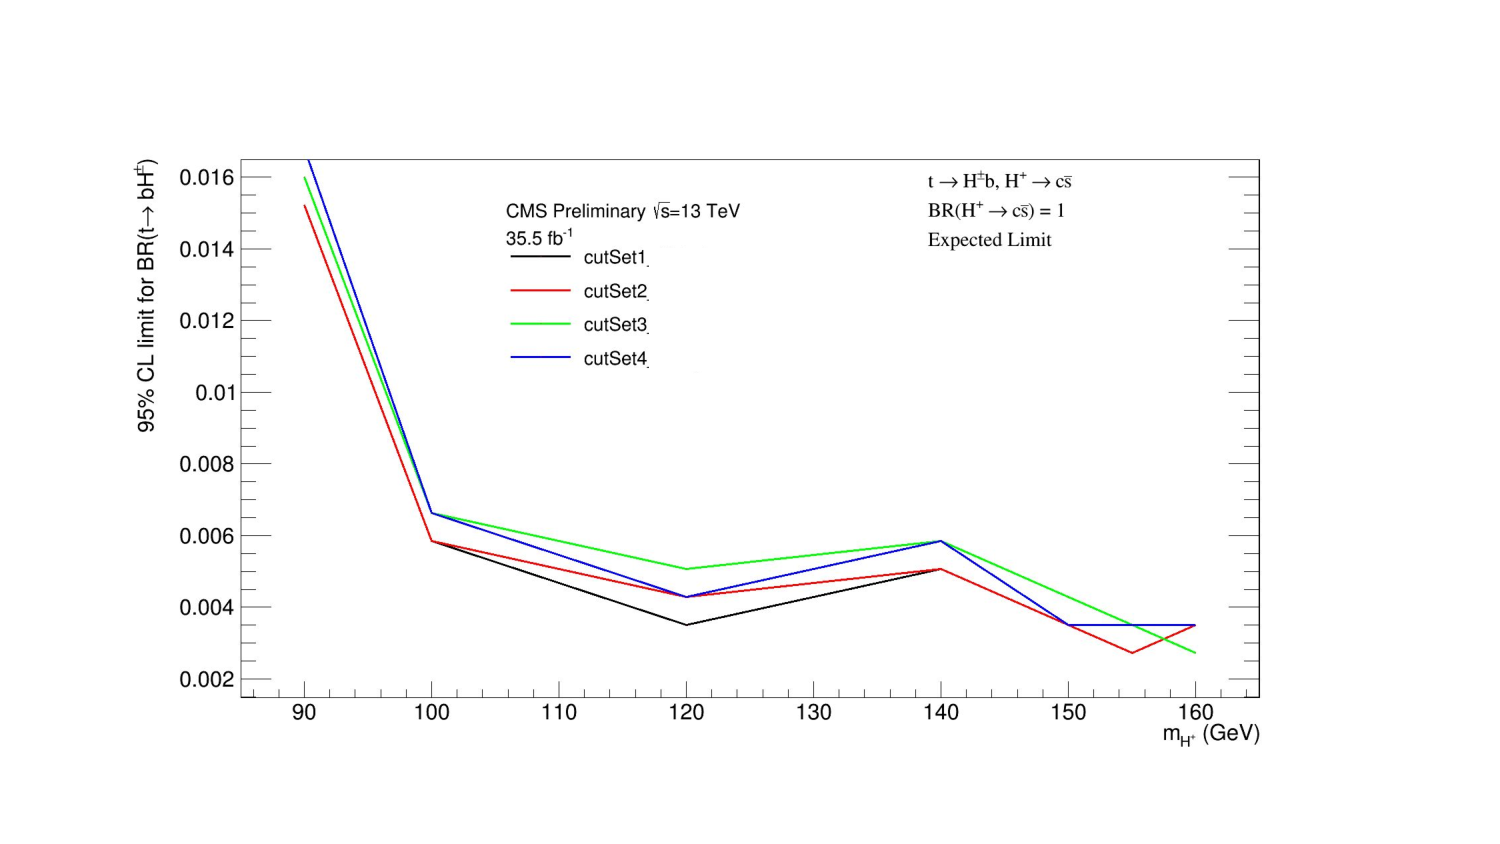
\includegraphics[width=0.70\textwidth]{Image/Limit/limit_cutset.pdf}
\caption{ The exclusion limit on ${\cal{BR}}(t \rightarrow b H^+)$ as a function of charged Higgs mass for different combination
of cuts listed in Table~\ref{tab:limit_cutset}. The exclusion limit of cut set-1 is better compared to that from other sets.}
\label{fig:limit_cutset}
\end{center}
\end{figure}


